\section{Paradigma \emph{Greedy}}

\subsection{Introduzione}

Il problema del memorylessness del paradigma \emph{Divide and Conquer} è stato risolto utilizzando il paradigma del \emph{Dynamic Programming}. Risolvendo un problema con la programmazione dinamica, però, la soluzione viene costruita componendo le soluzioni di sottoistanze, scegliendo di volta in volta la sottosoluzione migliore. Questa scelta può avvenire solo dopo aver calcolato \emph{tutte} le soluzioni alle sottoistanze.

Il paradigma \emph{Greedy} seleziona ad ogni iterazione la scelta più promettente, e calcola la soluzione alla sottoistanza relativa \emph{solo} a quella scelta.

Occorre dimostrare che la scelta non comprometta l'ottimalità della soluzione.

\subsection{Definizione}

Il paradigma \emph{Greedy} agisce in tre passi:
\begin{enumerate}
    \item Scelta \emph{Greedy}: compie una scelta che sembra essere quella più promettente, localmente ottima, che non comprometta la soluzione: la soluzione ottima conterrà quella scelta.
    \item \emph{Clean up}: l'istanza viene ripulita, in accordo con la scelta effettuata.
    \item \emph{Tail recursion}: viene risolta l'\emph{unica} istanza generata, come ultimo comando della funzione. Questo tipo di ricorsione può sempre essere scritto in maniera iterativa.
\end{enumerate}

Vanno quindi dimostrate due proprietà:
\begin{enumerate}
    \item la scelta \emph{Greedy} (SG) non compromette l'ottimalità della soluzione locale: \\
        $\exists S^*$ che contiene la scelta \emph{Greedy}
    \item $\exists S^*$ che, oltre alla scelta \emph{Greedy}, contiene la soluzione della sottoistanza ottenuta dal \emph{clean up}, detta sottoistanza residua
\end{enumerate}

\section{Selezione di attività}

\subsection{Definizione del problema}

Un problema che si presta ad essere risolto con il paradigma \emph{Greedy} è la selezione di attività. Data una risorsa condivisa e un insieme di attività che la utilizzano, come si può selezionare il massimo numero di attività compatibili? Formalmente si definiscono:
\begin{itemize}
    \item[--] Risorsa condivisa
    \item[--] Insieme di attività $S = \left\{ a_1, \cdots, a_n \right\}$ con $a_i = [s_i, f_i)$
    \item[--] Attività compatibili: $a_i$ è compatibile con $a_j$ se
        $[s_i, f_i) \cap [s_j, f_j) = \emptyset$
        o
        $(f_i \leq s_j ) \vee (f_j \leq s_i)$
\end{itemize}
L'obiettivo è determinare il sottoinsieme $S^* \subseteq S$ di attività mutualmente compatibili (intervalli a coppie disgiunti) di cardinalità massima.

\subsection{Soluzione \emph{Greedy}}

Senza perdita di generalità, si può assumere che le attività siano ordinate per tempo di fine non decrescente:
$f_1 \leq f_2 \leq \cdots \leq f_n$

L'intuizione è di selezionare di volta in volta l'istanza che finisce prima, in modo da lasciare il più tempo possibile \emph{compatto} per selezionare le altre. Nella fase di \emph{clean-up}, si scorrono le attività in ordine, eliminando quelle non compatibili. È sufficiente fermarsi alla prima istanza compatibile che si trova: successive istanze che non sono compatibili con quella selezionata, non saranno compatibili neppure con quella trovata per prima, e saranno eliminate successivamente.

\begin{algorithm}[H]
\caption{Selezione di attività, implementazione ricorsiva}\label{alg:asrec}
\begin{algorithmic}[1]
    \Procedure{REC\_AS}{$\vec{s}, \vec{f}, g$}
        \State $n \gets \vec{s}.len$
        \If{$g > n$}
        \Comment{Problema vuoto}
            \State return
        \EndIf
        \State $SG \gets \left\{ a_g \right\}$
        \Comment{Prima attività, scelta \emph{Greedy}}
        \State $i \gets g+1$
        \While{ $\left( s_i < f_g \right) \wedge \left( i \leq n \right)$}
            \State $i \gets i+1$
            \Comment{\emph{Clean-up}}
        \EndWhile
        \State return $SG \cup \Call{REC\_AS}{\vec{s}, \vec{f}, i}$
        \Comment{\emph{Tail recursion}}
    \EndProcedure
\end{algorithmic}
\end{algorithm}

\begin{algorithm}[H]
\caption{Selezione di attività, implementazione iterativa}\label{alg:asiter}
\begin{algorithmic}[1]
    \Procedure{GREEDY\_AS}{$\vec{s}, \vec{f}$}
        \State $n \gets \vec{s}.len$
        \State $g \gets 1$
        \State $A \gets \left\{ a_g \right\}$
        \Comment{Insieme di attività scelte $A$}
        \For{$i \gets 2 $ to $ n $ }
        \Comment{Alterna selezione e \emph{clean-up}}
            \If{$ s_i \geq f_g $}
                \State $g \gets i$
                \State $A \gets A \cup \left\{ a_g \right\}$
            \EndIf
        \EndFor
        \State return $A$
    \EndProcedure
\end{algorithmic}
\end{algorithm}

\subsection{Dimostrazione della correttezza}

\subsubsection{Proprietà di scelta \emph{Greedy}}

Occorre dimostrare che esiste una soluzione ottima $A^*$ che contiene la scelta \emph{Greedy} ${a_1}$. Si procede per \emph{cut and paste}: Sia $\widehat{A}$ una soluzione ottima. Se ${a_1} \in \widehat{A}$ si conclude, se no si sostituisce un'attività in $\widehat{A}$ con la scelta \emph{Greedy} e si dimostra che l'insieme ottenuto è ancora ottimo e contiene la scelta \emph{Greedy}.
Sia $\widehat{i} =  \argmin\limits_i \{ a_i \in \widehat{A} \} $, e sia
\[
A^* = \widehat{A} 
\;
\underbracket[1pt]{
\setminus \left\{ a_{\widehat{i}} \right\} 
}_{\text{\emph{cut}}}
\;
\underbracket[1pt]{
\vphantom{ \setminus \left\{ a_{\widehat{i}} \right\} }
\cup \left\{ a_1 \right\}
}_{\text{\emph{paste}}}
\]

Va dimostrato che $a_1$ è compatibile con ogni $a_j$, ossia 
$\forall a_j \in \widehat{A} \setminus \left\{ a_{\widehat{i}} \right\} \Rightarrow f_1 \leq s_j$
\\
Vale $f_1 \leq f_{\widehat{i}}$ perché $a_1$ è la scelta \emph{Greedy}, e $f_{\widehat{i}} \leq s_j$ perché $\widehat{A}$ contiene attività compatibili, per cui $f_1 \leq s_j$, e $A^*$ è ammissibile. Inoltre $|A^*| = |\widehat{A}|$, quindi è anche soluzione ottima. Per costruzione $A^*$ contiene la scelta \emph{Greedy}, e si conclude.

\subsubsection{Proprietà di sottostruttura ottima}

Va dimostrata l'esistenza di una soluzione ottima $A^*$ che, oltre ad $a_1$, contiene una soluzione ottima al sottoproblema residuo $S_r$. 
Il sottoproblema residuo si ottiene effettuando il \emph{clean-up}, eliminando tutte le attività $a_j$, con $j>1$, per cui $s_j < t_1$, fermandosi o per $g : f_1 \leq s_g$, o quando tutte le attività sono state eliminate. $S_r$ è quindi un suffisso di attività che parte da $g$.

Si possono verificare due casi:

$S_r = \emptyset $: tutte le attività sono in conflitto con $a_1 \Rightarrow A^*=\left\{ a_1 \right\}$
e la soluzione al $S_r$ è $sol( A^* \setminus \left\{ a_1 \right\} ) = sol ( \emptyset ) = \emptyset$.
La soluzione al $S_r$ è vuota, e $A^*$ oltre alla scelta \emph{Greedy} non contiene nulla.

$S_r = \left\{ a_g, a_{g+1}, \cdots, a_n \right\}, g>1$: almeno un'attività è compatibile con $a_1$, la soluzione ottima dovrà contenere almeno due attività. Si deve dimostrare che $A^* \setminus \left\{ a_1 \right\}$ è soluzione ammissibile e ottima per $S_r$.

Per dimostrare l'ammissibilità vanno mostrate due proprietà: le attività in $A^* \setminus \left\{ a_1 \right\}$ devono essere mutualmente compatibili, e lo sono perché questo è un sottoinsieme di attività compatibili; $A^* \setminus \left\{ a_1 \right\} \subseteq S_r$, devono essere attività contenute in $S_r$, e lo sono, perché $S_r$ è stato ottenuto proprio eliminando $a_1$ e tutte le attività non compatibili con questa, ossia $a_2, \cdots, a_{g-1}$, e nessuna delle attività eliminate per ottenere $S_r$ potrebbe convivere con $a_1$.

Per dimostrare l'ottimalità di $A^* \setminus \left\{ a_1 \right\}$ per $S_r$ si procede per assurdo, supponendo che $A^* \setminus \left\{ a_1 \right\}$ \emph{non} sia ottima per $S_r$. Deve quindi esistere un sottoinsieme $\widehat{A} \subseteq S_r$ di attività compatibili
contenente $a_g$, la scelta \emph{Greedy} per $S_r$,
con $|\widehat{A}| > |A^*|-1$, e se questo fosse vero si troverebbe una soluzione a $S$ migliore di $A^*$, che era ottima.
Si può aggiungere a questo insieme $a_1$ che di sicuro non è già presente, non essendo in $S_r$, ottenendo $|\widehat{A} \cup \left\{ a_1 \right\} | > |A^*|$. 
Tutte le attività in $\widehat{A}$ sono compatibili con $a_1$, infatti $f_1 < s_g$ per costruzione del problema residuo, $s_g < f_g$ per ogni attività e $f_g < s_i$ per ogni attività in $\widehat{A}$, per la compatibilità di $a_g$.
Questo conduce ad un assurdo, perché $A^*$ era la soluzione ottima.

\section{Compressione di un file}

\subsection{Definizione del problema}

Un file può essere visto come stringa di caratteri di un alfabeto, $F \in \Sigma^*$. A ciascun carattere è associata una frequenza: $\forall c \in \Sigma : f(c) \in [0,1]$. Il file usa solo un sottoalfabeto $C \subseteq \Sigma : c \in C \Rightarrow f(c) > 0$.

La compressione è una mappa che associa ad ogni carattere una stringa di bit:
\[
    % l_F : \Sigma \rightarrow \left\{ 0,1 \right\}^* \\
    e : C \rightarrow \left\{ 0,1 \right\}^*
\]

Le $e(c)$ sono dette parole di codice, o \emph{codeword}.
Le mappe di codifica sono memorizzate in una struttura detta \emph{trie}, un albero binario etichettato.
Per ricostruire il file originale, è sufficiente mantenere due puntatori, uno sul trie e uno sul file codificato, scorrendo il file e scendendo l'albero, tornando alla radice ogni volta che si arriva ad una foglia.

Un esempio di file, codificato con caratteri ASCII a 8 bit, è caratterizzato dalle frequenze dei caratteri che compaiono nel file:
\begin{equation*}
    \begin{array}[H]{rcccccc}
        \texttt{C:} & a & b & c & d & e & f \\
        \texttt{freq rel:} & 0.45 & 0.13 & 0.12 & 0.16 & 0.09 & 0.05
    \end{array}
\end{equation*}
Se $|F| = 100M$ caratteri, per memorizzarlo senza compressione sono necessari $800 Mbit$. Il file usa solo 6 dei 256 caratteri possibili, sono quindi sufficienti meno bit per memorizzarli. In generale, per memorizzare $k$ caratteri sono necessari $\left\lceil \log_2 k \right\rceil$ bit. In questo caso, 3 bit sono sufficienti, e il file si può quindi memorizzare con $300 Mbit$ utilizzando una codifica a lunghezza costante (\emph{fixed-length encoding}).
\begin{equation*}
    \begin{array}[H]{rcccccc}
        \texttt{C:} & a & b & c & d & e & f \\
        \texttt{codifica:} & 000 & 001 & 010 & 011 & 100 & 101
    \end{array}
\end{equation*}
Oltre al file compresso occorre memorizzare anche la mappa di codifica, ma la sua dimensione è generalmente irrisoria rispetto a quella del file.
In \rfig{tree:lungcost} è mostrato il \emph{trie} della codifica a lunghezza costante.
\begin{figure}[h]
\begin{center}
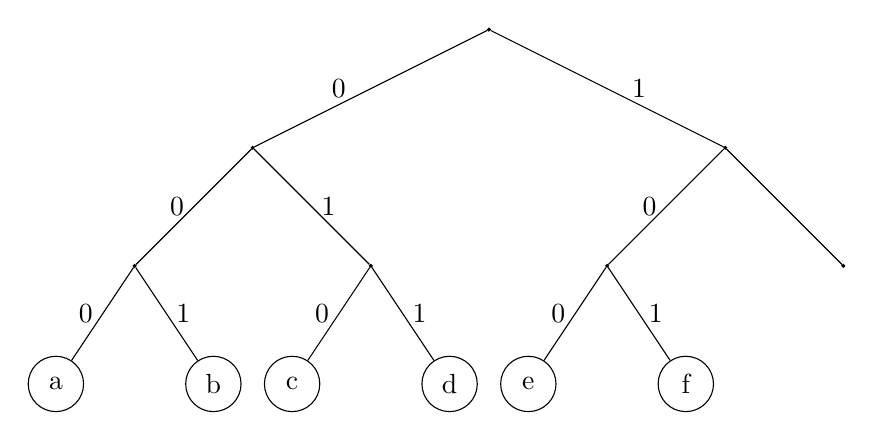
\begin{tikzpicture}[
        level/.style={sibling distance=60mm/#1},
        redge/.style={right,draw=none},
        ledge/.style={left,draw=none},
        inner/.style={draw,circle,fill=black,inner sep=0pt,minimum width=0pt},
        % inner/.style={inner sep=0pt,minimum width=0pt},
        % inner/.style={inner sep=0pt,minimum width=-1pt},
        leaf/.style={circle,draw,minimum width=20pt},
        ]
    \node (z) [inner] {}
    child {
        node [inner] (a) {}
        child {
            node [inner] (b) {}
                child {
                    node [leaf] (b1) {a}
                    edge from parent node[ledge] {0}
                }
                child {
                    node [leaf] (b2) {b}
                    edge from parent node[redge] {1}
                }
            edge from parent node[ledge] {0}
        }
        child {
            node [inner] (e) {}
                child {
                    node [leaf] (e2) {c}
                    edge from parent node[ledge] {0}
                }
                child {
                    node [leaf] (e2) {d}
                    edge from parent node[redge] {1}
                }
            edge from parent node[redge] {1}
        }
        edge from parent node[ledge] {0$\;\;$} % edge da (a)
    }
    child {
        node [inner] (c) {}
        child {
            node [inner] (d) {}
                child {
                    node [leaf] (d1) {e}
                    edge from parent node[ledge] {0}
                }
                child {
                    node [leaf] (d2) {f}
                    edge from parent node[redge] {1}
                }
            edge from parent node[ledge] {0}
        }
        child {
            node [inner] (c2) {}
            % edge from parent node[redge] {1}
        }
        edge from parent node[redge] {$\;\;$1}
    }
    ; % end of the node
\end{tikzpicture}
\end{center}
\caption{\emph{Trie} della codifica a lunghezza costante}
\label{tree:lungcost}
\end{figure}
Questo \emph{trie} è chiaramente non ottimo: una delle foglie non è utilizzata.
Assegnare ancora meno bit ad alcune lettere può condurre ad una compressione ancora maggiore, ma bisogna assicurarsi che la codifica risultante sia libera da prefissi (\emph{prefix code}). Per esempio la seguente codifica
\begin{equation*}
    \begin{array}[H]{rcccccc}
        \texttt{C:} & a & b & c & d & e & f \\
        \texttt{codifica:} & 0 & 00 & 01 & 1 & 10 & 11
    \end{array}
\end{equation*}
non permette di distinguere $e(`ad \textit{'})$ e $e(`c \textit{'})$.
Questa codifica però fornisce il limite inferiore alla grandezza possibile del file compresso:
\begin{equation*}
    |F| \left( 0.45*1 + 0.13*2 + \dots \right) = 153M
\end{equation*}
Per assicurare la decodificabilità deve valere
\begin{equation*}
    \nexists \, c_1, c_2 : e(c_1) \text{ è prefisso di } e(c_2)
\end{equation*}
Si definisce profondità di un carattere $c$ in un \emph{trie} la quantità $d_T(c) = |e(c)|$.
\\
Il costo di una codifica è
\begin{equation*}
    \sum_{c \in C}\left( |F| f(c) \right) d_T(c) = 
    |F| \sum_{c \in C} f(c) d_T(c) = 
    |F| B(T)
\end{equation*}
dove $B(T)$ è la somma della profondità delle foglie del \emph{trie} pesata con le frequenze del carattere. $B(T)$ è anche la lunghezza di \emph{codeword} media.
\\
L'obiettivo è minimizzare $B(T)$ su tutti i possibili \emph{trie} per l'insieme di caratteri $C$.

\subsection{Soluzione \emph{Greedy}}

\subsubsection{Proprietà di un \emph{trie} ottimo}

Prima di poter arrivare alla soluzione, si deve dimostrare la seguente proprietà: un \emph{trie} ottimo $T^*$ per $\{C,f\}$ è sempre un albero binario pieno.

La dimostrazione si svolge per assurdo, ipotizzando che esista un albero ottimo \emph{non} pieno. In questo caso deve esistere un nodo $u$ con un solo figlio $v$. Questo nodo è radice di un sottoalbero, che ha come foglia $c'$ (se fosse composto solo da $v$, $c'$ è scelto coincidente con $v$).
\\
Si possono unire i due nodi $u$ e $v$ in un singolo nodo, ottenendo l'albero $\widehat{T}$. Questo è un albero ammissibile per $\{C,f\}$, infatti non scompaiono foglie, e vale
\begin{equation*}
    \forall c \in C : d_{T^*} (c) \geq d_{\widehat{T}} (c)
\end{equation*}
Infatti al di fuori del sottoalbero resta tutto inalterato, mentre per le foglie del sottoalbero la profondità scende di 1, e questo succede per \emph{almeno} una foglia $c'$: $d_{\widehat{T}} (c') = d_{T^*} (c') -1$
\begin{align*}
    B \left( \widehat{T} \right)
    &= \sum_{c \in C} d_{\widehat{T}} (c) f(c) \\
    &= \sum_{c \in C \setminus \left\{ c' \right\}} d_{\widehat{T}} (c) f(c) + d_{\widehat{T}} (c') f(c') \\
    &\leq \sum_{c \in C \setminus \left\{ c' \right\}} d_{T^*} (c) f(c) 
    + d_{T^*} (c') f(c') - f(c') \\
    &= \sum_{c \in C} d_{T^*} (c) f(c) - f(c') \\
    &= B \left( T^* \right) - f(c')
\end{align*}
Ma questo è assurdo perché $f(c')>0$, avendo scartato i caratteri a costo nullo, e $T^*$ era l'albero ottimo.

Si può quindi riscrivere l'albero a lunghezza fissa come

\begin{figure}[h]
\begin{center}
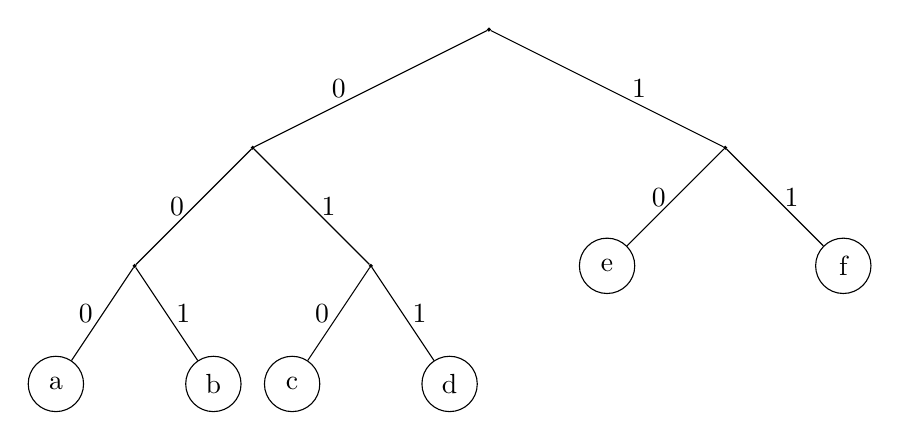
\begin{tikzpicture}[
        level/.style={sibling distance=60mm/#1},
        redge/.style={right,draw=none},
        ledge/.style={left,draw=none},
        inner/.style={draw,circle,fill=black,inner sep=0pt,minimum width=0pt},
        % inner/.style={inner sep=0pt,minimum width=0pt},
        % inner/.style={inner sep=0pt,minimum width=-1pt},
        leaf/.style={circle,draw,minimum width=20pt},
        ]
    \node (z) [inner] {}
    child {
        node [inner] (a) {}
        child {
            node [inner] (b) {}
                child {
                    node [leaf] (b1) {a}
                    edge from parent node[ledge] {0}
                }
                child {
                    node [leaf] (b2) {b}
                    edge from parent node[redge] {1}
                }
            edge from parent node[ledge] {0}
        }
        child {
            node [inner] (e) {}
                child {
                    node [leaf] (e2) {c}
                    edge from parent node[ledge] {0}
                }
                child {
                    node [leaf] (e2) {d}
                    edge from parent node[redge] {1}
                }
            edge from parent node[redge] {1}
        }
        edge from parent node[ledge] {0$\;\;$} % edge da (a)
    }
    child {
        node [inner] (c) {}
            child {
                node [leaf] (d1) {e}
                edge from parent node[ledge] {0}
            }
            child {
                node [leaf] (d2) {f}
                edge from parent node[redge] {1}
            }
        edge from parent node[redge] {$\;\;$1}
    }
    ; % end of the node
\end{tikzpicture}
\end{center}
\caption{\emph{Trie} subottimo ricavato dalla codifica a lunghezza costante}
\label{tree:lungcostimproved}
\end{figure}

\subsubsection{Soluzione \emph{Greedy}}
Si è quindi definito un problema di ottimizzazione molto chiaro: va determinato un albero pieno ottimo che minimizzi $B(T)$:
\begin{equation*}
    T^* = \argmin \left\{ B(T) : T \right\}
\end{equation*}
L'albero ottimo viene generato compiendo successive operazioni di \emph{merge} tra sottoalberi, creando di volta in volta un nuovo nodo interno.
Si inizia con $k=n=|C|$ alberi, e ad ogni iterazione si passa da $k$ a $k-1$ alberi. Dopo $n-1$ iterazioni si conclude, avendo ottenuto un singolo albero con $n$ foglie.

L'intuizione su cui si basa la scelta degli alberi da unire si basa sul fatto che quando si compie un \emph{merge} la profondità delle foglie dei sottoalberi coinvolti viene incrementata di 1: ha quindi probabilmente senso scegliere ogni volta le due con frequenza minore.
\\
Se $x$ e $y$ sono le due foglie con frequenza minore ($f(x)<f(y)<\dots$), dopo l'unione condividono tutto il prefisso e sono differenziate dall'ultimo carattere. Si può quindi considerare un unico pseudocarattere $z$ associato al prefisso, con $f(z) = f(x)+f(y)$. In questo modo si hanno $n-2$ caratteri non modificati e un carattere nuovo, generando un problema di taglia $n-1$.
\\
Per convenzione, si associa l'etichetta $0$ alla foglia con frequenza minore, e si chiama quel ramo \emph{sinistro}, indipendentemente dalla rappresentazione grafica.

Memorizzando le frequenze in una coda di priorità l'operazione di ricerca del minimo viene eseguita in $O(1)$ mentre l'inserimento di un nuovo nodo si compie in $O(\log n)$.

La classe nodo ha i seguenti attributi: $left$ e $right$ per memorizzare i nodi figli; per le foglie, viene memorizzato il valore speciale $nil$. $f$ indica la frequenza combinata del nodo; $char$, per le foglie, memorizza il carattere.

Si può quindi procedere alla scrittura dell'algoritmo di \emph{Huffman}.

\begin{algorithm}[H]
\caption{Algoritmo di \emph{Huffman}}\label{alg:huff}
\begin{algorithmic}[1]
    \Procedure{HUFFMAN}{$C, f$}
        \State $n \gets |C|$
        \State $Q \gets \emptyset$
        \ForAll{$c \in C$}
            \State $z \gets \Call{newnode}{ }$
            \State $z.f \gets f(c)$
            \State $z.char \gets c$
            \State $z.left \gets z.right \gets nil$
            \State $Q.insert(z)$
            \Comment{Le priorità in $Q$ sono le frequenze}
        \EndFor
        \For{$i \gets 1$ to $n-1$}
            \State $x \gets Q.\Call{extractmin}{ }$
            \State $y \gets Q.\Call{extractmin}{ }$
            \State $z \gets \Call{newnode}{ }$
            \State $z.left \gets x$
            \State $z.right \gets y$
            \State $z.f \gets x.f + y.f$
            \State $Q.\Call{insert}{z}$
        \EndFor
        \State return $Q.\Call{extractmin}{ }$
    \EndProcedure
\end{algorithmic}
\end{algorithm}

\begin{figure}[h]
\centering % to center the subfigures
% \begin{center}
\begin{subfigure}[b]{0.9\textwidth}
% \begin{center}
\centering % to center the tikzpicture
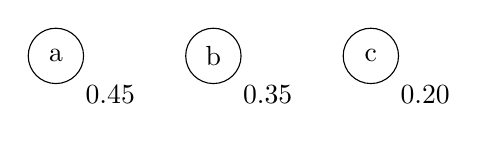
\begin{tikzpicture}[
        subtree/.style={draw,circle,minimum width=20pt},
        ]
    \node (a) [subtree, label=below right:{$0.45$}] at (0,0) {a};
    \node (b) [subtree, label=below right:{$0.35$}] at (2,0) {b};
    \node (c) [subtree, label=below right:{$0.20$}] at (4,0) {c};
\end{tikzpicture}
\caption{Iterazione 0}
\label{fig:huffit0}
% \end{center}
\end{subfigure}
\\
\begin{subfigure}[b]{0.9\textwidth}
\centering % to center the tikzpicture
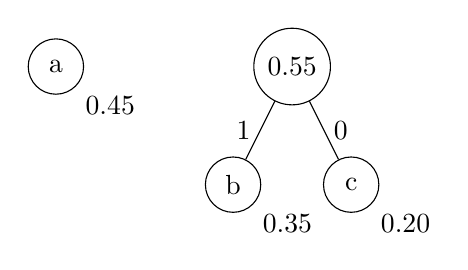
\begin{tikzpicture}[
        redge/.style={right,draw=none},
        ledge/.style={left,draw=none},
        subtree/.style={draw,circle,minimum width=20pt},
        ]
    \node (a) [subtree, label=below right:{$0.45$}] at (0,0) {a};
    \node (bc) [subtree] at (3,0) {$0.55$}
        child {
            node (b) [subtree, label=below right:{$0.35$}] {b}
            edge from parent node[ledge] {1}
        }
        child {
            node (c) [subtree, label=below right:{$0.20$}] {c}
            edge from parent node[redge] {0}
        }
    ; % end of bc
\end{tikzpicture}
\caption{Iterazione 1}
\label{fig:huffit1}
\end{subfigure}
\\
\begin{subfigure}[b]{0.9\textwidth}
\centering % to center the tikzpicture
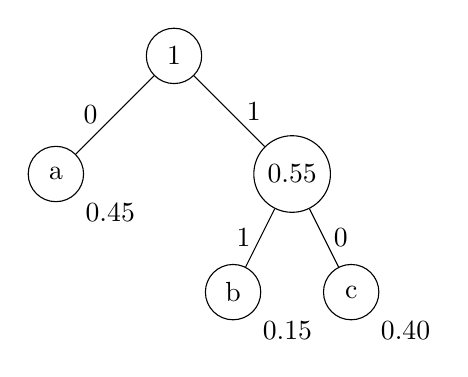
\begin{tikzpicture}[
        level/.style={sibling distance=30mm/#1},
        % level/.style={sibling distance=20mm},
        redge/.style={right,draw=none},
        ledge/.style={left,draw=none},
        subtree/.style={draw,circle,minimum width=20pt},
        inner/.style={inner sep=0pt,minimum width=9pt},
        ]
    \node (abc) [subtree] at (0,0) {$1$}
        child {
            node (a) [subtree, label=below right:{$0.45$}] {a}
            edge from parent node[ledge] {$0\;$}
        }
        child {
            node (bc) [subtree] {$0.55$}
            child {
                node (b) [subtree, label=below right:{$0.15$}] {b}
                edge from parent node[ledge] {1}
            }
            child {
                node (c) [subtree, label=below right:{$0.40$}] {c}
                edge from parent node[redge] {0}
            }
            edge from parent node[redge] {$\;1$}
        }
    ; % end of abc
\end{tikzpicture}
\caption{Iterazione 2}
\label{fig:huffit2}
\end{subfigure}
\caption{Iterazioni dell'algoritmo di Huffman}
\label{tree:treehuff}
\end{figure}

\subsection{Dimostrazione della correttezza}

\subsubsection{Proprietà di scelta \emph{Greedy}}

Va dimostrato che, se $x,y$ sono i due caratteri di frequenza minima ($f(x) \leq f(y) \leq \dots$), esiste un \emph{trie} ottimo $T^*$ in cui le foglie di $x$ ed $y$ sono sorelle.

Si consideri una generica soluzione ottima $\widehat{T}$ e si individuino le due foglie sorelle $w,z$ di massima profondità ($f(w) \leq f(z) \leq \dots$) (devono esistere perché è un albero pieno \emph{finito}). Si dimostra che sostituendo al loro posto $x,y$ non si peggiora la soluzione.

Possono capitare due casi: se $w=x \vee z=y$, si conclude. Se $w \neq x \wedge z \neq y$ vanno analizzati tre casi. Nel caso più generale, entrambi sono diversi e $x,y$ sono foglie nell'albero con profondità non massima. Si possono quindi scambiare di posto $x \leftrightarrow w$ e $y \leftrightarrow z$, sostituendo la parole di codice di $x$ con quella di $w$ e rispettivamente per $y$ e $z$. Se si dimostra che quest'albero è ancora ottimo, si conclude, avendo esibito un albero che è ottimo e contiene la scelta \emph{Greedy} ($x,y$ sorelle).

Si analizzi la differenza tra $B(\widehat{T})$ e $B(T^*)$, notando che per tutte le foglie che non sono $x,y,w,z$, la profondità non cambia.
\begin{align*}
    B(\widehat{T}) - B(T^*)
    &= \sum_{c \in C} f(c) d_{\widehat{T}} (c) - \sum_{c \in C} f(c) d_{T^*} (c) \\
    &=
      f(w) d_{\widehat{T}} (w)
    + f(x) d_{\widehat{T}} (x)
    + f(z) d_{\widehat{T}} (z)
    + f(y) d_{\widehat{T}} (y) 
    \\ &
    - f(x) d_{T^*} (x)
    - f(w) d_{T^*} (w)
    - f(y) d_{T^*} (y)
    - f(z) d_{T^*} (z) 
    \intertext{scambiando $d_{T^*} (x) \leftrightarrow d_{\widehat{T}} (w)$ e così via si ottiene}
    &=
      f(w) d_{\widehat{T}} (w)
    + f(x) d_{\widehat{T}} (x)
    + f(z) d_{\widehat{T}} (z)
    + f(y) d_{\widehat{T}} (y) 
    \\ &
    - f(x) d_{\widehat{T}} (w)
    - f(w) d_{\widehat{T}} (x)
    - f(y) d_{\widehat{T}} (z)
    - f(z) d_{\widehat{T}} (y) 
    \intertext{raccogliendo poi i $d_{\widehat{T}} (w)$ si ottiene}
    &=
      d_{\widehat{T}} (w) \left( f(w) - f(x) \right)
    - d_{\widehat{T}} (x) \left( f(w) - f(x) \right)
    \\ &+
      d_{\widehat{T}} (z) \left( f(z) - f(y) \right)
    - d_{\widehat{T}} (y) \left( f(z) - f(y) \right)
    \intertext{e raccogliendo ancora si ricava}
    &=
    \left( d_{\widehat{T}} (w) - d_{\widehat{T}} (x) \right)
    \left( f(w) - f(x) \right)
    \\ &+
    \left( d_{\widehat{T}} (z) - d_{\widehat{T}} (y) \right)
    \left( f(z) - f(y) \right)
    \intertext{i quattro fattori sono positivi: le profondità di $w,z$ sono maggiori di quelle di $x,y$, essendo stati scelti come nodi di profondità massima; le frequenze di $x,y$ sono minori di quelle di $w,z$, essendo i nodi con frequenza minima. Quindi}
    B(\widehat{T}) - B(T^*) &\geq 0
    \\
    B(T^*) &\leq B(\widehat{T})
    \intertext{ma $\widehat{T}$ è una generica soluzione ottima, non la si può migliorare, per cui}
    B(T^*) &= B(\widehat{T})
\end{align*}
Anche $T^*$ è quindi una soluzione ottima, e contiene la scelta \emph{Greedy}.

\subsubsection{Proprietà di sottostruttura ottima}

Va ora di mostrato che, dato $T^*$ che contiene la scelta \emph{Greedy}, quest'albero contiene anche un \emph{trie} $T'$, ottimo per il sottoproblema residuo. Il residuo è caratterizzato da
\begin{align*}
    \text{alfabeto} \quad &
    C \setminus \left\{ x,y \right\} \cup \left\{ z \right\} \\
    \text{frequenze} \quad & 
    f(c) = 
    \begin{cases}
        f(c) & c \in C \setminus \left\{ x,y \right\} \\
        f(x) + f(y) & c=z
    \end{cases}
\end{align*}
E $T'$ si ricava da $T^*$ potando le due foglie $x,y$ e sostituendole con $z$. Si consideri la relazione tra i costi dei due alberi:
\begin{align*}
    B(T^*) 
    &= \sum_{c \in C} f(c) d_{T^*} (c) \\
    &= \sum_{c \in C \setminus \left\{ x,y \right\}} f(c) d_{T^*} (c)
    + f(x) d_{T^*} (x)
    + f(y) d_{T^*} (y)
    \intertext{essendo alla stessa profondità si può raccogliere $d_{T^*} (x)$}
    &= \sum_{c \in C \setminus \left\{ x,y \right\}} f(c) d_{T^*} (c)
    + d_{T^*} (x) \left( f(x) + f(y) \right)
    \intertext{applicando la distributiva, sommando e sottraendo $1$}
    &= \sum_{c \in C \setminus \left\{ x,y \right\}} f(c) d_{T^*} (c)
    + \left( d_{T^*} (x) -1 \right)
    \left( f(x) + f(y) \right)
    + \left( f(x) + f(y) \right)
    \intertext{tutti i nodi che non sono $x,y,z$ non variano di profondità, e vale
        $d_{T^*} (x) -1 = d_{T'} (z)$
    }
    &= \sum_{c \in C \setminus \left\{ x,y \right\}} f(c) d_{T'} (c)
    + d_{T'} (z) f(z) + f(z)
    \\
    &= \sum_{c \in C \setminus \left\{ x,y \right\} \cup \left\{ z \right\}} f(c) d_{T'} (c)
    + f(z)
    \intertext{la frequenza è positiva e costante, per cui si ricava una relazione lineare tra i costi}
    B(T^*) &= B(T') + cost.
\end{align*}
Si dimostra che la relazione lineare comporta l'ottimalità di $T'$, procedendo per \emph{cut and paste}: se $T'$ non fosse ottimo, lo si potrebbe sostituire con $T'' : B(T'') < B(T')$. Da $T''$ si ricava $\widehat{T}$ sostituendo a $z$ le foglie $x,y$, ottenendo una soluzione per il problema originale.
\begin{equation*}
    B(\widehat{T}) = B(T'') + f(z) < B(T') + f(z) = B(T^*)
\end{equation*}
Ma $T^*$ era ottimo, e la supposizione che $T'$ non lo fosse ha condotto ad un assurdo.

% \
% \subsection{autocomplete}
% Snippet di \LaTeX{} che non ho voglia di cercare nei file

% Una bella scatola:
% \begin{equation}
    % \boxed{x^2+y^2 = z^2}
% \end{equation}

% Numeri nei casi
% \begin{numcases}{T(n)=}
    % 2^3 \label{escaso1} \\
    % 2^4 \label{escaso2} 
% \end{numcases}

% Sotto numeri
% \begin{subnumcases}{T(n)=}
    % 2^3 \label{escaso3} \\
    % 2^4 
% \end{subnumcases}

% Liste compatte
% \begin{itemize}[noitemsep,topsep=0pt,parsep=0pt,partopsep=0pt]
    % \item qualcosa
    % \item[+] qualcosa
    % \item[*] qualcosa
    % \item[--] qualcosa
% \end{itemize}

% Parole in libertà per l'autocomplete: 
% à
% è
% ì
% ò
% ù
% perché
% così
% sì
% può
% più

% Viva vim se scrivi \verb|<C-k>`e| o \verb|<C-k>e`| in insert mode mette una è

% % delirio doppio di vim se scrivi \verb|<C-k>da| in insert mode mette ``Hiragana letter DA'' che purtroppo non posso mostrarvi %だ
% % insomma i digraph sono tanti e belli

% Spazietti fra equazioni
% \begin{equation*}
    % A^{[0]}(x) = \sum_{j=0}^{\frac{n}{2}-1} a_{2j}x^j
    % \quad \text{ e } \quad
    % A^{[1]}(x) = \sum_{j=0}^{\frac{n}{2}-1} a_{2j+1}x^j
% \end{equation*}

% Un gustoso algoritmo
% \begin{algorithm}[H]
% \caption{Divide and Conquer}\label{alg:dncmock}
% \begin{algorithmic}[1]
    % \Procedure{D\&C}{$i$}
        % \If{$|i| \leq n_0$}                             \Comment{BASE}
            % \State *risolvo direttamente*
        % \EndIf
        % \State $<i_1, i_2, \dots, i_k> \gets A_D(i)$    \Comment{DIVIDE}
        % \For{$j \gets 1 $ to $ k $ }                    \Comment{RECURSE}
            % \State $s_j \gets $ \Call{D\&C}{$i_j$}
        % \EndFor
        % \State $s \gets A_C(<s_1, s_2, \dots, s_k>)$    \Comment{CONQUER}
        % \State return $s$
    % \EndProcedure
% \end{algorithmic}
% \end{algorithm}

% Un alberello
% \begin{center}
% \begin{tikzpicture}[
        % level/.style={sibling distance=60mm/#1},
        % redge/.style={right,draw=none},
        % ledge/.style={left,draw=none},
        % inner/.style={draw,circle,fill=black,inner sep=0pt,minimum width=0pt},
        % % inner/.style={inner sep=0pt,minimum width=0pt},
        % % inner/.style={inner sep=0pt,minimum width=-1pt},
        % leaf/.style={circle,draw},
        % ]
    % \node (z) [inner] {}
    % child {
        % node [inner] (a) {}
        % child {
            % node [inner] (b) {}
                % child {
                    % node [leaf] (b1) {left}
                    % edge from parent node[ledge] {0}
                % }
                % child {
                    % node [leaf] (b2) {righ}
                    % edge from parent node[redge] {1}
                % }
            % edge from parent node[ledge] {0}
        % }
        % child {
            % node [inner] (e) {}
                % child {
                    % node [leaf] (e2) {left}
                    % edge from parent node[ledge] {0}
                % }
                % child {
                    % node [leaf] (e2) {righ}
                    % edge from parent node[redge] {1}
                % }
            % edge from parent node[redge] {1}
        % }
        % edge from parent node[ledge] {0} % edge da (a)
    % }
    % child {
        % node [inner] (c) {}
        % child {
            % node [inner] (d) {}
                % child {
                    % node [leaf] (d1) {left}
                    % edge from parent node[ledge] {0}
                % }
                % child {
                    % node [leaf] (d2) {righ}
                    % edge from parent node[redge] {1}
                % }
            % edge from parent node[ledge] {0}
        % }
        % child {
            % node [inner] (f) {}
                % child {
                    % node [leaf] (f1) {left}
                    % edge from parent node[ledge] {0}
                % }
                % child {
                    % node [leaf] (f2) {righ}
                    % edge from parent node[redge] {1}
                % }
            % edge from parent node[redge] {1}
        % }
        % edge from parent node[redge] {1}
    % }
  % ; % end of the node
% \end{tikzpicture}
% \end{center}
